%\documentclass[iop]{emulateapj}
\documentclass[aps, pre, onecolumn, nofootinbib, notitlepage, groupedaddress, amsfonts, amssymb, amsmath, longbibliography]{revtex4-1}
\usepackage{graphicx}
\usepackage{hyperref}
\usepackage{xcolor}
\hypersetup{
    colorlinks,
    linkcolor={red!50!black},
    citecolor={blue!50!black},
    urlcolor={blue!80!black}
}
\usepackage{bm}
\usepackage{natbib}
\usepackage{longtable}
\LTcapwidth=0.87\textwidth

\newcommand{\Div}[1]{\ensuremath{\nabla\cdot\left( #1\right)}}
\newcommand{\DivU}{\ensuremath{\nabla\cdot\bm{u}}}
\newcommand{\angles}[1]{\ensuremath{\left\langle #1 \right\rangle}}
\newcommand{\grad}{\ensuremath{\nabla}}
\newcommand{\RB}{Rayleigh-B\'{e}nard }
\newcommand{\stressT}{\ensuremath{\bm{\bar{\bar{\Pi}}}}}
\newcommand{\lilstressT}{\ensuremath{\bm{\bar{\bar{\sigma}}}}}
\newcommand{\nrho}{\ensuremath{n_{\rho}}}
\newcommand{\approptoinn}[2]{\mathrel{\vcenter{
	\offinterlineskip\halign{\hfil$##$\cr
	#1\propto\cr\noalign{\kern2pt}#1\sim\cr\noalign{\kern-2pt}}}}}

\newcommand{\appropto}{\mathpalette\approptoinn\relax}

\newcommand\mnras{{MNRAS}}%

\begin{document}
\author{Evan H. Anders}
\affiliation{Dept. Astrophysical \& Planetary Sciences, University of Colorado -- Boulder, Boulder, CO 80309, USA}
\affiliation{Laboratory for Atmospheric and Space Physics, Boulder, CO 80303, USA}
\author{Benjamin P. Brown}
\affiliation{Dept. Astrophysical \& Planetary Sciences, University of Colorado -- Boulder, Boulder, CO 80309, USA}
\affiliation{Laboratory for Atmospheric and Space Physics, Boulder, CO 80303, USA}
\author{Jeffrey Oishi}
\affiliation{Bates}
\title{Accelerated convergence of convective simulations using boundary value problems}

\begin{abstract}
WOW this is a really long sentence check out this abstract I'll just keep writing words to make this at least
one line long so we know what the formatting looks like, ok?
\end{abstract}
\maketitle


\section{Introduction}
\label{sec:intro}
Natural convection occurs in the presence of disparate timescales. Granules on the
solar surface overturn on the order of 10 minutes, whereas deep motions in the Sun are likely at
low Mach number and constrained by the solar rotation rate of \~1 month.  
Despite these relatively short dynamical times, the scale of energy transport on the
Sun occurs on the Kelvin-Helmholtz timescale of nearly $3 \times 10^7$ \emph{years} \cite{stix2003}. 
As simulations aim to model natural convection
by increasing into the high-Rayleigh Number (Ra) regime, where diffusive timescales are much
longer than dynamical timescales \cite{Anders&Brown2017}, achieving converged simulations will 
require runs which span a greater number of convective timescales in order to thermally converge.
Furthermore, with increasing Ra and decreasing diffusivities, motions become more turbulent
and require finer grid meshes and smaller timesteps to resolve turbulent motions, meaning that
achieving even one overturn timescale becomes a harder problem.  
These two effects combine to make thermally converging high-Ra, astrophysically interesting
simulations intractable using modern numerical tools.

In studies of stratified convection where a convective layer lies between stable layers, studies
have used the knowledge of Mixing Length Theory (MLT) to adjust the initial thermal profile of
atmospheres to a state which is closer to the adiabat chosen by convection \cite{brandenburg&all2005}.
However, many studies of convection do not contain stable layers above and below the convection
zone, and the presence of hard boundaries and the boundary layers that they form means
that the proper adiabat cannot be known \emph{a priori} until the simulation evolves the
structure of the boundary layers.

The chosen boundary conditions at the upper and lower plates
determine key quantities of the dynamics of the evolved state.
Studies of incompressible, Boussinesq, \RB convection (RBC) often
employ fixed temperature (Dirichlet) or fixed heat flux
(Neumann) boundary conditions at both plates.  
Dirichlet conditions represent plates of infinite conductivity,
whereas Neumann conditions model plates of finite conductivity.  
In both cases, choosing symmetric boundary conditions maintains overall system symmetry, 
and despite evolving towards different thermal structures, both types of conditions
transport heat in the same manner \cite{johnston&doering2009}.

Studies of convection which aim to model
in astrophysical systems, such as the outer envelopes of low-to-moderate mass stars 
like the Sun, often employ a mixture of these
two types of boundary conditions \cite{hurlburt&all1984, cattaneo&all1991, korre&all2017}.  
The flux at the lower boundary is fixed, modeling
the constant energy generation of the stellar core, 
while the outer boundary condition is held at a fixed temperature,
modeling the surface of a star which must output the energy generated internally.
While this setup is a useful model for understanding natural
systems, simulations which employ this setup often suffer from a long 
thermal relaxation as the atmosphere loses energy and approaches the adiabat chosen by the
Dirichlet condition.

Here we present a method for using simple boundary value problems (BVPs), 
along with information about the evolved flow fields,
to fast-forward the slow thermal evolution of convecting simulations.  
We run two sets of experiments: one in which we allow convective simulations to evolve for a
full thermal timescale before taking measurements, and another in which we employ a fast-forwarding,
BVP technique which occurs on dynamical timescales. We compare these two sets of simulations to
show the validity of the BVP technique.  Then, we use the BVP technique to run simulations
at high Ra, in the regime where running for thermal timescales becomes computationally intractable.

\section{Experiment}
\label{sec:experiment}
In our study, we adopt the Oberbeck-Boussinesq approximation.  Here, the
fluid has constant kinematic viscosity ($\nu$), thermal diffusivity ($\kappa$), and coefficient
of thermal expansion ($\alpha$).  We non-dimensionalize length by the layer height ($L_z$) ,
temperature by the (constant) initial temperature gradient across the layer ($\grad T_0$), and time
by the freefall timescale ($L_z / v_{\text{ff}}$, with $v_{\text{ff}} = \sqrt{\alpha g L_z^2 \grad T_0}$, where $g$ is 
uniform gravitational acceleration in the $-\hat{z}$ direction). The dimensionless Boussinesq
equations governing the velocity $\bm{u} = u\hat{x} + v\hat{y} + w\hat{z}$, temperature
$T = T_0 + T_1$, and reduced pressure $\varpi$ are \cite{spiegel&veronis1960}
\begin{gather}
\DivU = 0, 
	\label{eqn:incompressible}
\\
\frac{\partial \bm{u}}{\partial t} + \bm{u}\cdot\grad\bm{u} =
-\grad\varpi + T_1\hat{z} + \frac{\text{Pr}}{\text{Ra}}\grad^2\bm{u}, 
	\label{eqn:bouss_momentum}
\\
\frac{\partial T_1}{\partial t} + \bm{u}\cdot\grad(T_0 + T_1) = \frac{1}{\text{Pr}\,\text{Ra}}\grad^2 T_1,
	\label{eqn:bouss_energy}
\end{gather}
where the dimensionless control parameters are the Rayleigh and Prandtl numbers,
\begin{equation}
\text{Ra} = \frac{g \alpha L^4 \left(\frac{dT}{dz}\right)_0}{\nu\chi} = \frac{(L\,v_{\text{ff}})^2}{\nu\chi}, \qquad \text{Pr} = \frac{\nu}{\chi}.
\end{equation}
The dimensionless vertical extent of the domain is $z = [-1/2, 1/2]$, and at the boundaries
we impose no-slip, impenetrable boundary conditions such that $w = u = v = 0$ at $z = \pm 1/2$.
At the lower boundary, we employ a fixed flux condition such that $\partial T_1 / \partial z = 0$
at $z = -1/2$, and we impose a fixed temperature condition $T_1 = 0$ at $z = 1/2$. Both
horizontal directions are periodic and have equal aspect ratio, $\gamma = 4$, such that
the horizontal coordinates $x, y = [0, \Gamma]$.


\subsection{The Boundary Value Problem}
\begin{figure}[b]
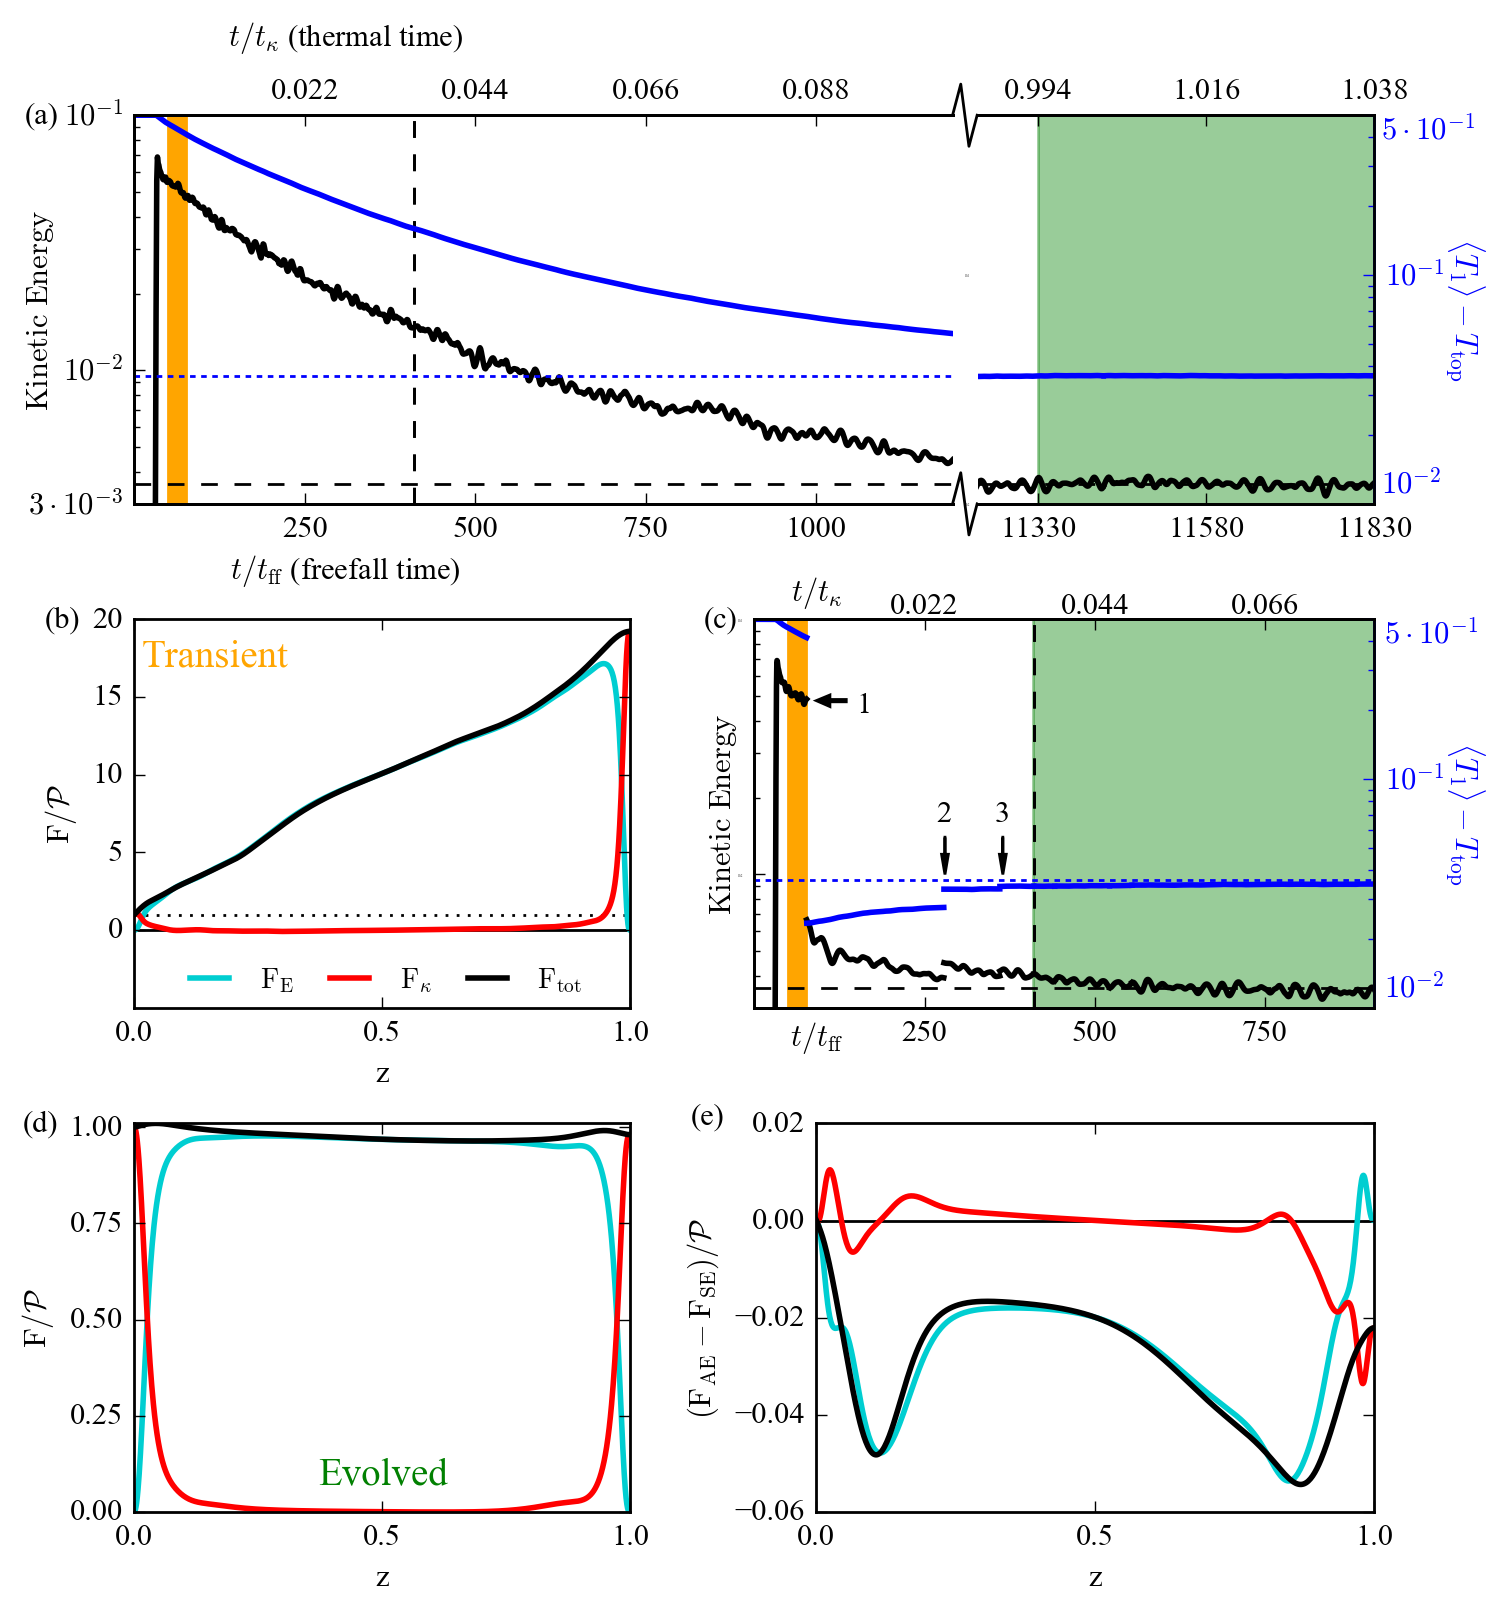
\includegraphics[width=\textwidth]{./figs/time_trace.png}
\caption{\label{fig:time_trace} }
\end{figure}

One can skip the prohibitive thermal timescale required to reach an equilibrium temperature profile
in a Direct Numerical Simulation (DNS) by coupling the DNS with a simple Boundary Value Problem
(BVP) solve. Using information about the dynamics of the convection in the atmosphere, it is possible
to skip a large portion of the thermal evolution, see Fig \ref{fig:time_trace}a\&b.

The Boussinesq BVP contains equations of hydrostatic balance and thermal equilibrium,
\begin{gather}
\frac{\partial}{\partial z}\angles{\varpi} = \angles{T_1}\hat{z},
	\label{eqn:bouss_BVP_momentum}
\\
\frac{\partial}{\partial z}\angles{wT_1} = \frac{1}{\text{Pr}\text{Ra}}\frac{\partial^2}{\partial z^2} \angles{T_1},
	\label{eqn:bouss_BVP_energy}
\end{gather}
where $\angles{A}$ represents a time- and horizontally averaged profile of the quantity $A$.  
These
equations arise from taking time- and horizontal- averages of Eqns (\ref{eqn:bouss_momentum}-\ref{eqn:bouss_energy})
and neglecting terms that vanish due to symmetry in the evolved flows.  Convective flows
are perturbations around a thermal profile defined by these equations in the proper evolved state.

In Boussinesq RBC, the thermal structure of the atmosphere is fully determined by the specification
of the convective flux, $F_{conv} = \angles{w T_1}$.  If this profile is known, then $T_1$ and
$\varpi$ can be found under the proper specifications of boundary conditions.  
Under the choice of mixed thermal boundary conditions, the initial
atmosphere contains more thermal energy ($\propto T$) than the 
evolved adiabatic solution.  As the atmosphere adjusts to be nearly isothermal in the interior,
it must evolve towards the (cold) temperature value specified at the upper boundary.
The evolution of the atmosphere results in an asymmetric flux profile during 
the slow thermal evolution of the atmosphere (Fig. \ref{fig:time_trace}c).  

In order to find the evolved temperature profile of the atmosphere using the Boussinesq BVP equations, 
the evolved profile of the convective flux must be properly specified.  In order to construct
this profile, we acknowledge that the evolved solution will in flux equilibrium, 
carrying the amount of the flux entering through the bottom.  
Thus, the steady-state profile of the convective flux can be approximated as
\begin{equation}
F_{\text{conv, steady}} = F_{\text{bot}}\frac{\angles{wT_1}}{\angles{wT_1 - \kappa \partial_z (T_0 + T_1)}}
= F_{\text{bot}}\frac{\angles{F_{\text{conv, IVP}}}}{\angles{F_{\text{tot, IVP}}}}.
\label{eqn:bouss_BVP_fconv}
\end{equation}
Or, put simply, the steady state convective flux is retrieved by properly removing the asymmettry
from the flux profile.

In our Boussinesq BVPs, we solve Eqns. (\ref{eqn:bouss_BVP_momentum}-\ref{eqn:bouss_BVP_energy}),
substituting $\angles{wT_1} = F_{\text{conv, steady}}$ as defined in eqn. (\ref{eqn:bouss_BVP_fconv})
to retrieve the proper vertical profile of $T_1$ and $\varpi$.  We then update the mean horizontal value
of $T_1$ and $\varpi$ in a corresponding IVP, and continue to timestep forward with the newly adjusted
atmosphere.

In essence, solving the BVP is equivalent to saying that even though the magnitude of flux through
the system is not initially correct, the system appropriately picks out the ratios
\begin{equation}
f_{\text{conv}} = \frac{F_{\text{conv}}}{F_{\text{tot}}}\qquad
f_{\text{cond}} = \frac{F_{\text{cond}}}{F_{\text{tot}}}.
\end{equation}
in the convective, transient state, but the total amount of flux is too large until the system
reaches the proper isotherm.  This procedure seems to converge the atmosphere quite well
(Fig. \ref{fig:time_trace}d\&e).




\subsection{Numerics}
We utilize the 
Dedalus\footnote{\url{http://dedalus-project.org/}} 
pseudospectral framework \cite{burns&all2016} to time-evolve  
(\ref{eqn:incompressible})-(\ref{eqn:bouss_energy}) 
using an implicit-explicit (IMEX), third-order, four-step 
Runge-Kutta timestepping scheme RK443 \cite{ascher&all1997}.  
The temperature field is decomposed as $T = T_0(z) + T_1(x, y, z, t)$
and the velocity is $\bm{u} = w\bm{\hat{z}} + u\bm{\hat{x}} + v\bm{\hat{y}}$.
In our 2D runs, $v = 0$.
Variables are time-evolved on a dealiased Chebyshev (vertical)
and Fourier (horizontal, periodic) domain in which the
physical grid dimensions are 3/2 the size of the coefficient grid.  
Domain sizes range from
32x128 coefficients at the lowest values of 
Ra to 1024x4096 coefficients at Ra $> 10^{9}$ in 2D.

As initial conditions, we fill $T_1$ with
random white noise whose magnitude is $10^{-6}(\text{Ra Pr})^{-1/2}$.
This ensures that the initial perturbations are much smaller than the
evolved convective temperature perturbations, even at large Ra.
We filter this noise spectrum in coefficient space, 
such that only the lower 25\% of the coefficients
have power.

In 2D, there are often multiple steady state solutions (e.g., 2-roll and 3-roll
solutions) which have slightly different flow properties (heat transport, etc.).
Even though the initial perturbations are very small, they shape the convective
transient and thus determine the nature of the steady state convection, at least in
the laminar regime.  In order to ensure that our results are not biased by differences
in flow structure, we ran the simulations using distinct random temperature perturbations
so as to compare statistics in comparable flow fields.  In 3D, rolls are nonstationary over
convective timescales, and so these effects need not be considered there.

\subsection{Results}
We use the standard definition of the Nusselt number,
\begin{equation}
\text{Nu} = \frac{\angles{wT - (\text{Ra Pr})^{-1/2}\grad T}}{\angles{- (\text{Ra Pr})^{-1/2} \grad T}} =
1 + \frac{\angles{wT}}{-\Delta T}\sqrt{\text{Ra Pr}},
\end{equation}
where $\Delta T = T(z = 1/2) - T(z = -1/2)$ is the evolved temperature difference
between the top and bottom plates.  This form of the Nusselt number is valid even when
the system is not yet in flux equilibrium, and reduces to the standard fixed flux definition
of Nu  = $[1 - \angles{wT} / P]^{-1}$ \cite{johnston&doering2009}.

Here we talk about how the solutions are different, or similar.  This includes:
\begin{enumerate}
\item Showing that the flow fields look similar
\item Showing how the temperature / flux profiles look similar/different
\item showing how Nu and Re scale with Ra in BVP / IVP.
\item showing how the PDFs of $w$, $wT$, and $T$ change.
\end{enumerate}

\begin{figure}[t]
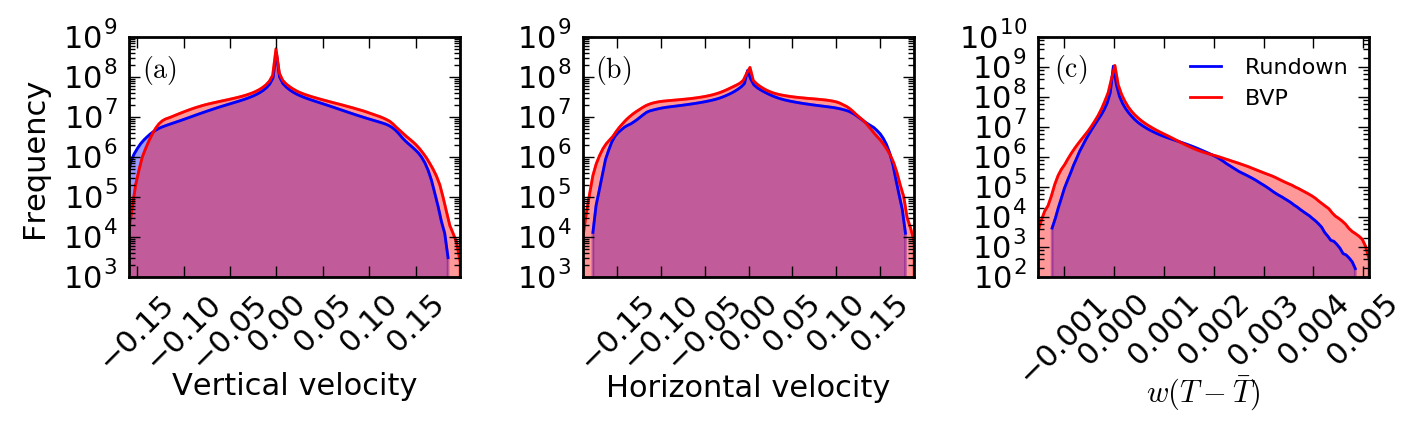
\includegraphics[width=\textwidth]{./figs/pdf_comparison.png}
\caption{\label{fig:pdf_comparison} }
\end{figure}

\begin{figure}[t]
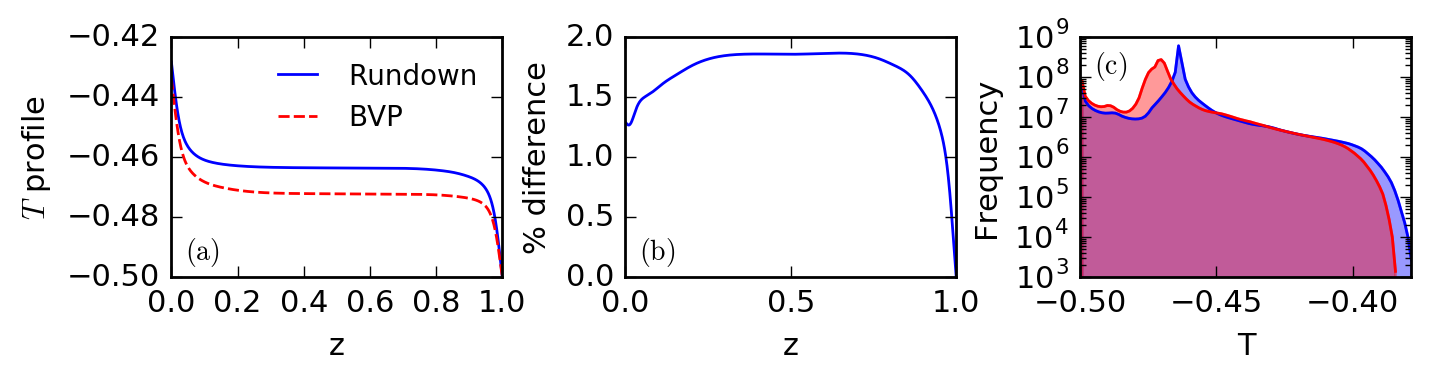
\includegraphics[width=\textwidth]{./figs/temp_comparison.png}
\caption{\label{fig:temp_comparison} }
\end{figure}

\begin{figure}[t]
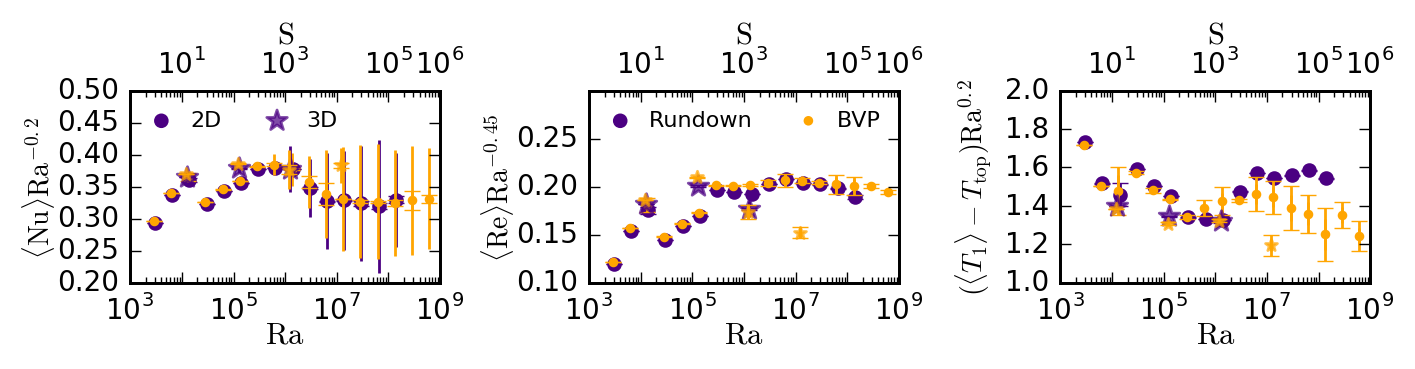
\includegraphics[width=\textwidth]{./figs/parameter_space_comparison.png}
\caption{\label{fig:parameter_space_comparison} }
\end{figure}





Then we need to make some comments about whether this is good or bad

Then we need to mention how the same thing can be done in stratified, just there you don't
assume symmetrical boundary layers.





\section{Discussion \& Conclusions}
\label{sec:results}




\begin{acknowledgments}
EHA acknowledges the support of the University of Colorado's George 
Ellery Hale Graduate Student Fellowship.
This work was additionally supported by  NASA LWS grant number NNX16AC92G.  
Computations were conducted 
with support by the NASA High End Computing (HEC) Program through the NASA 
Advanced Supercomputing (NAS) Division at Ames Research Center on Pleiades
with allocations GID s1647 and GID g26133.
\end{acknowledgments}


\appendix
\section{Table of Boussinesq Runs}



\section{Table of stratified runs}


\bibliography{biblio.bib}
\end{document}
